\documentclass[journal,twoside,web]{ieeecolor}
\usepackage{generic}
\usepackage{cite}
\usepackage{amsmath,amssymb,amsfonts}
\usepackage{algorithmic}
\usepackage{graphicx}
\usepackage{algorithm,algorithmic}
\usepackage{hyperref}
\hypersetup{hidelinks=true}
\usepackage{textcomp}
% added packages
\usepackage{subcaption}
\graphicspath{{Fig/}}
\usepackage{booktabs}
\usepackage[flushleft]{threeparttable}
\usepackage{placeins}
%\usepackage{natbib}
\usepackage[flushleft]{threeparttable}
\usepackage{placeins}

\def\BibTeX{{\rm B\kern-.05em{\sc i\kern-.025em b}\kern-.08em
    T\kern-.1667em\lower.7ex\hbox{E}\kern-.125emX}}
\markboth{\hskip25pc IEEE TRANSACTIONS AND JOURNALS TEMPLATE}
{Author \MakeLowercase{\textit{et al.}}: Title}
\begin{document}
\title{Supplementary material for\\ DruGNNosis-MoA: Elucidating Drug Mechanisms as Etiological or Palliative With Graph Neural Networks Employing a Large Language Model}
\author{
%Brettler Liad, 
%Berman Eden,
%Jagodnik Kathleen M.,
%and 
%Bartal Alon
\thanks{
%This paragraph of the first footnote will contain the date on 
%All authors are with the The School of Business Administration, Bar-Ilan University, Ramat-Gan, 5290002, Israel (e-mail: alon.bartal@biu.ac.il).
}
}

\maketitle

%Full names of authors are preferred in 

%the author field, but are not required.

%Put a space between authors' initials.

%The abstract must be between 150--250 words. 

% three or four different keywords or phrase

%---------------------------------------------------------------------
\appendices
%---------------------------------------------------------------------
%\begin{appendices}

\setcounter{figure}{0}
\renewcommand\thefigure{S\arabic{figure}} % Redefine table numbering style

%-------------------
\section{Supplementary Figures}
%-------------------
\begin{figure}[h!]
    \centering
    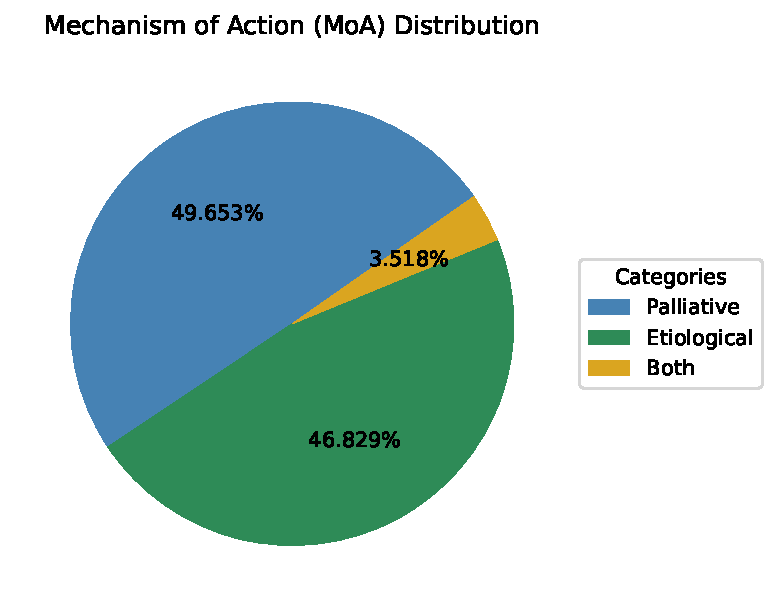
\includegraphics[width=\linewidth]{Figures/EvsP.pdf}
    \caption{Distribution of drug mechanisms of action. The number of etiological and palliative drugs is well balanced, with 47.423\% (957) being etiological, and 48.761\% (984) being palliative.
    Only a small percentage (3.816\%, 77) of drugs exhibit both mechanisms.}
    \label{fig:EvsP}
\end{figure}

%-------------------

\begin{figure}[h!]
    \centering
    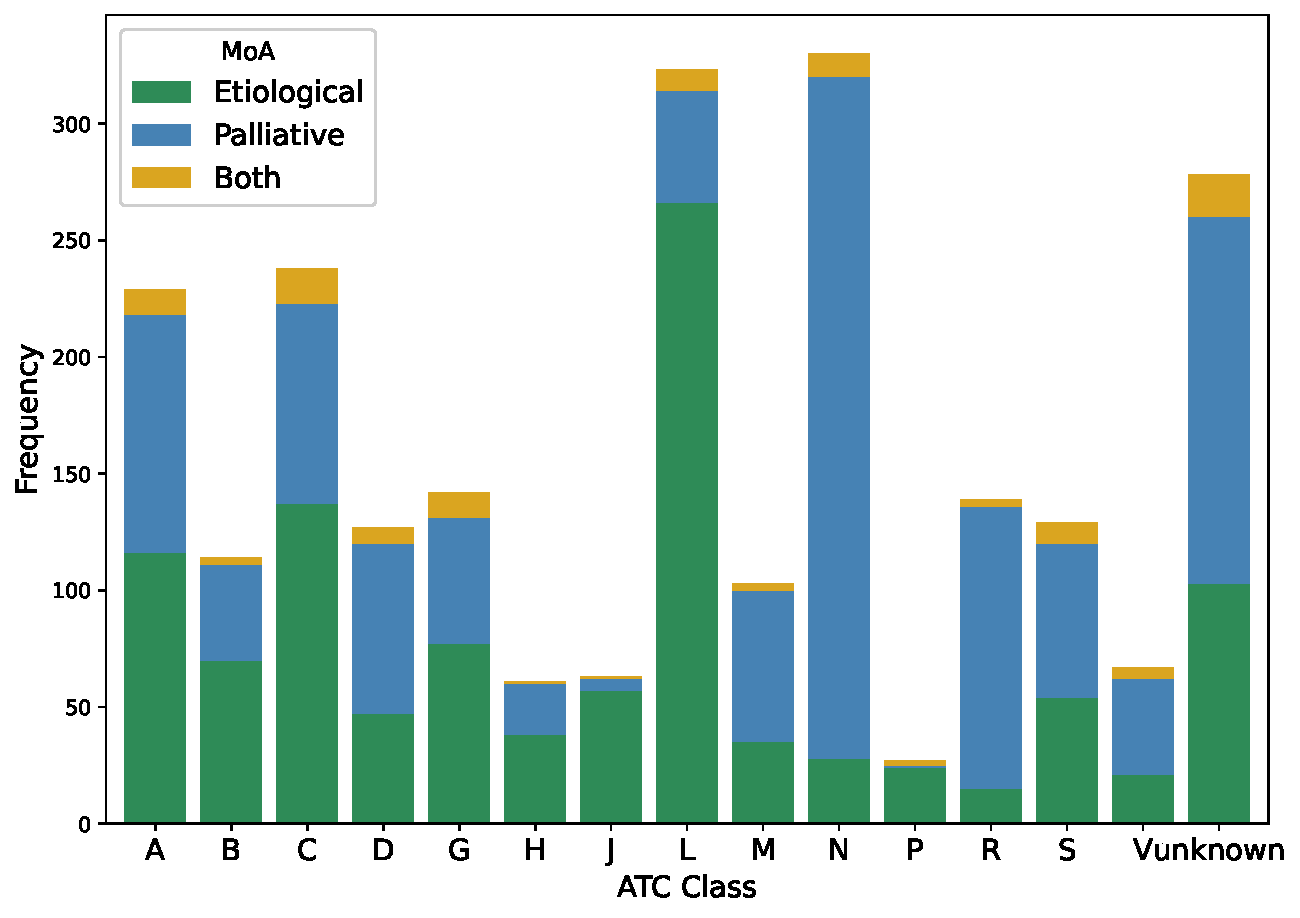
\includegraphics[width=\linewidth]{Figures/EPvsATC.pdf}
    \caption{ Distribution of drug mechanisms across Anatomical Therapeutic Chemical (ATC) classes.
    Each ATC class has a unique distribution of drug mechanisms.
    Some classes, e.g., `J', `L', and `P', are mainly associated with drugs having etiological mechanisms.
    In contrast, classes like 'N' and `R' are primarily associated with drugs having palliative mechanisms.
    The remaining classes generally exhibit a balance between drugs with etiological and palliative mechanisms.
    ATC Class Definitions:
   ``A": Alimentary tract and metabolism;
   ``B": Blood and blood forming organs;
   ``C": Cardiovascular system;
   ``D": Dermatologicals;
   ``G": Genito urinary system and sex hormones;
   ``H": Systemic hormonal preparations, excluding sex hormones and insulins;
   ``J": Antiinfectives for systemic use;
   ``L": Antineoplastic and immunomodulating agents;
   ``M": Musculo-skeletal system;
   ``N": Nervous system;
   ``P": Antiparasitic products, insecticides and repellents;
   ``R": Respiratory system;
   ``S": Sensory organs;
   ``V": Various;
   "Unknown": Drug entries that do not have an ATC class assigned to them in DrugBank.
    }
    \label{fig:EPvsATC}
\end{figure}

%-------------------

\begin{figure}
\centering
\begin{subfigure}{\linewidth}
   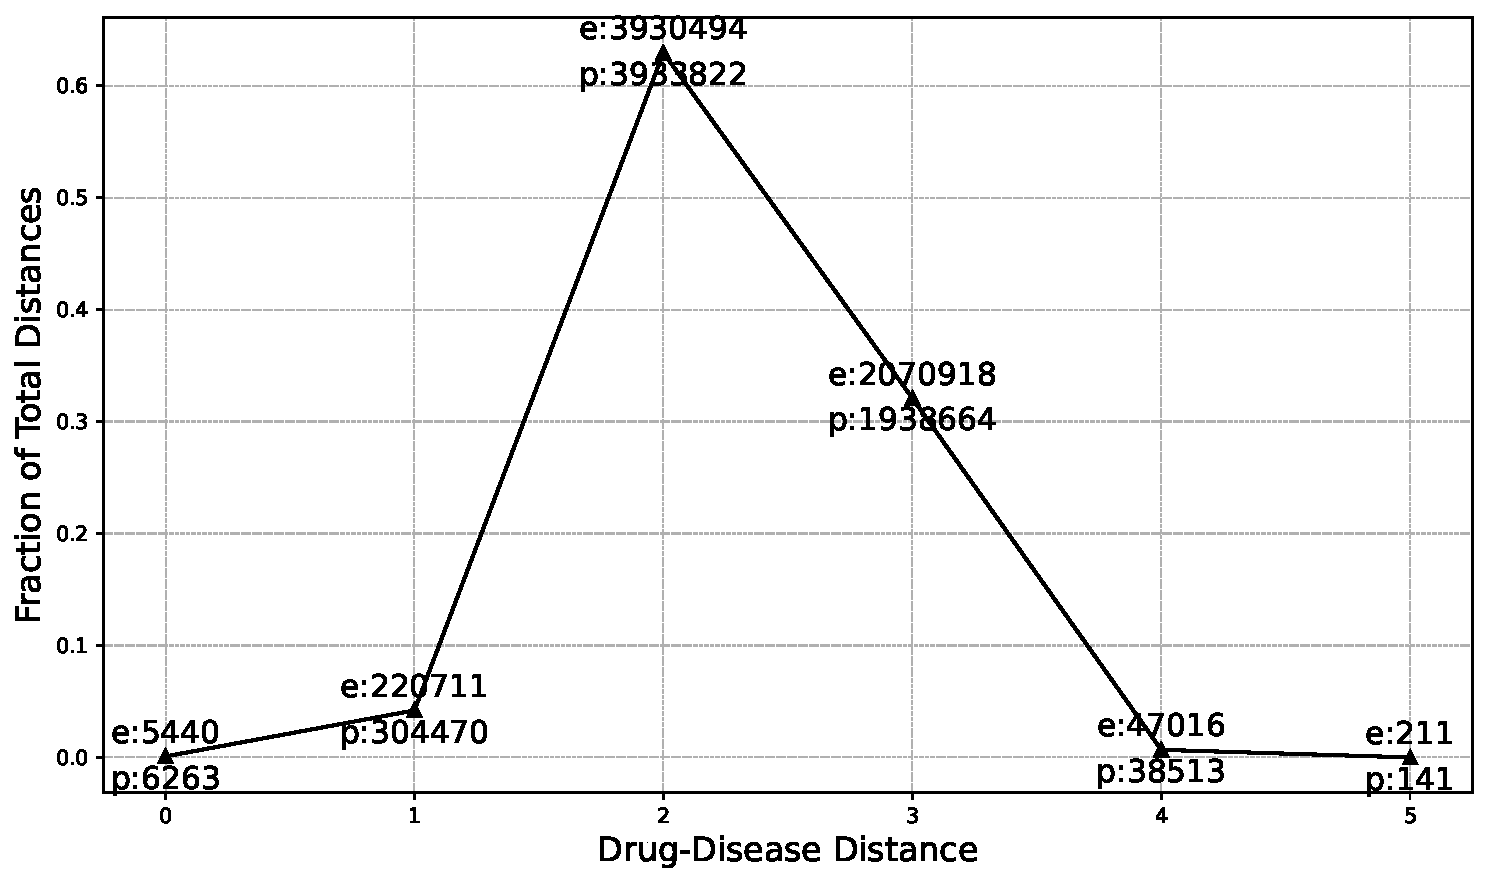
\includegraphics[width=\linewidth]{Figures/Yildrim_all_shortest_distance.pdf}
   \caption{\textbf{All vs. All (Comprehensive) Method:} Calculates and counts the shortest distance between each drug and disease pair, considering each occurrence of the drug in multiple paths.
   According to the technique of [5], 
   %\cite{yildirim2007drug}
   distances 0 and 1 hold statistical significance and are considered to indicate etiological drug mechanisms.}
   \label{fig:yildirim1}
\end{subfigure}
\begin{subfigure}{\linewidth}
   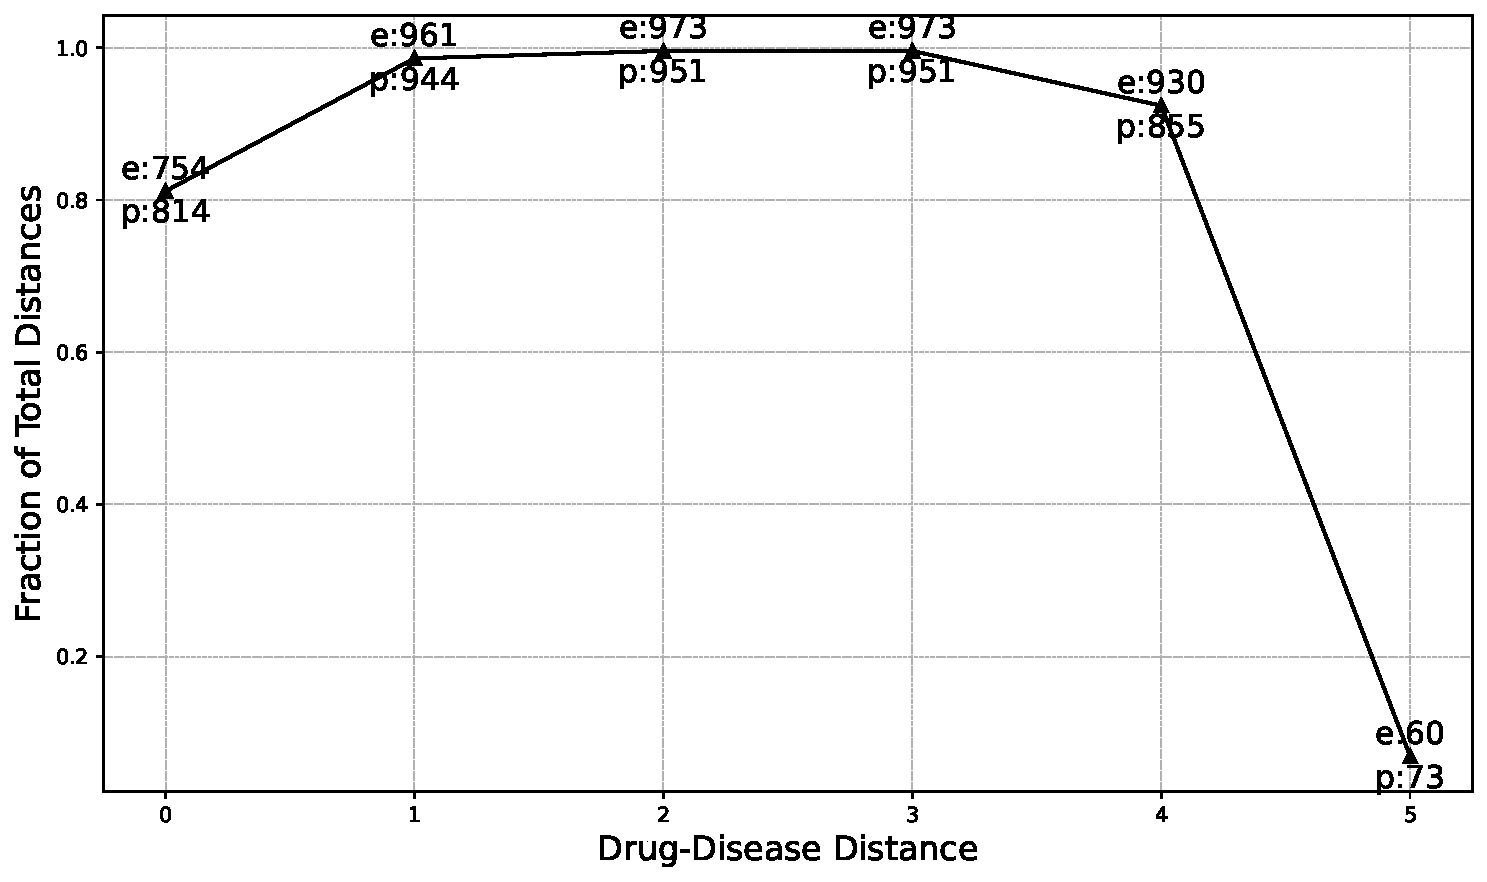
\includegraphics[width=\linewidth]{Figures/Yildrim_ALL_unique_drug_count_shortest_distance.pdf}
   \caption{\textbf{All vs. All (Unique) Method:} 
   Calculates the shortest distances between each drug and disease pair using a distinct counting mechanism. A drug is counted only once at each unique distance, regardless of how many times it appears at that distance. This ensures a balanced representation of drug applications relative to distance, preventing overemphasis on drugs appearing multiple times at the same distance.}
   \label{fig:yildirim2}
\end{subfigure}
\begin{subfigure}{\linewidth}
   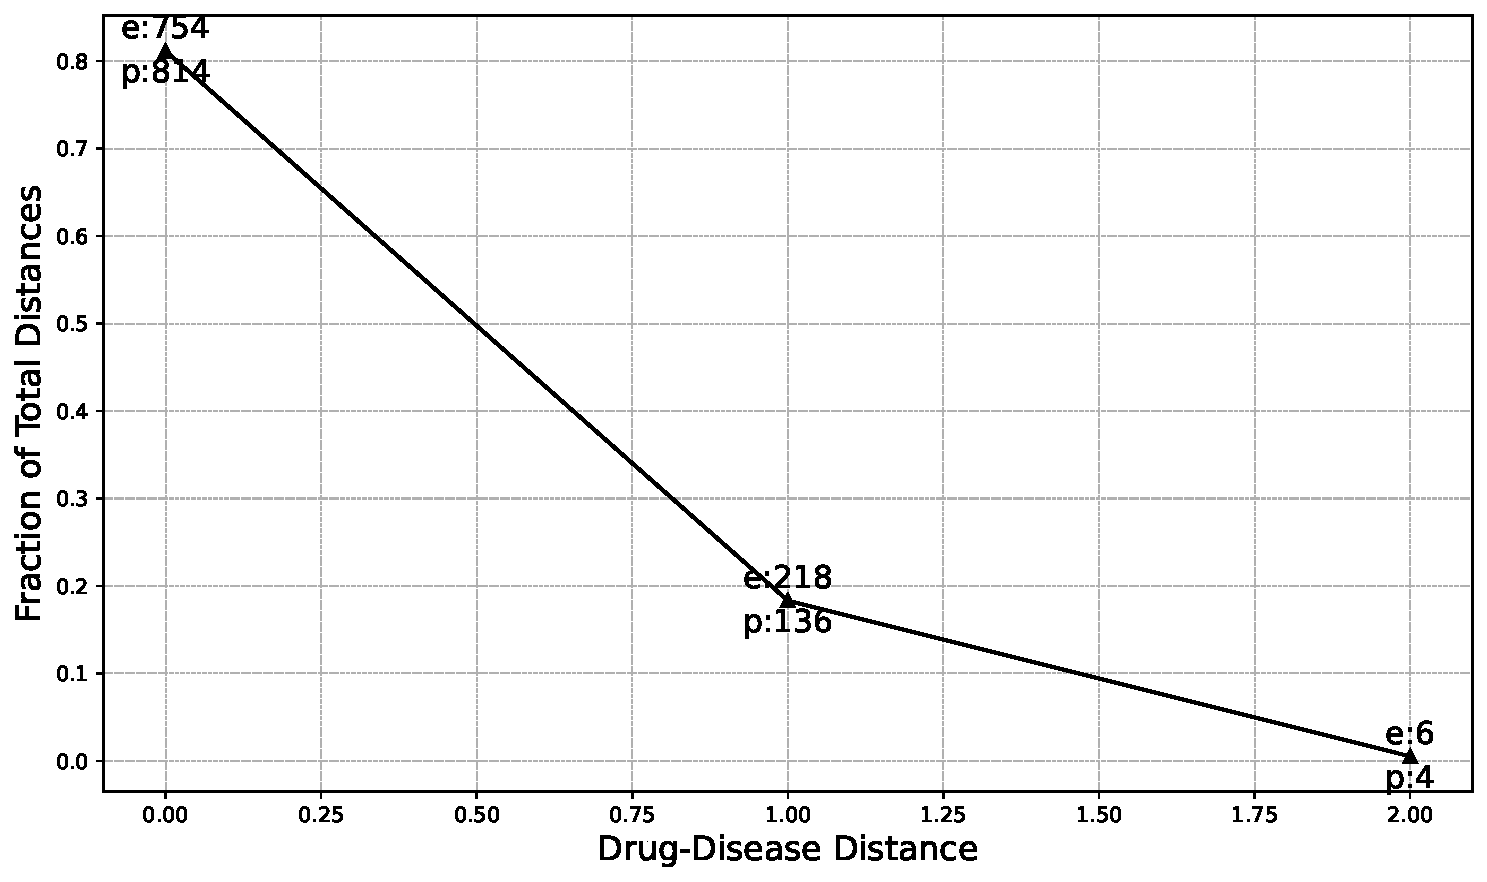
\includegraphics[width=\linewidth]{Figures/Yildrim_unique_minimum_shortest_distance.pdf}
   \caption{\textbf{Unique Minimum Shortest Distance Method:} 
   For each drug, we identified its shortest distance to a disease. 
   If a drug had the same shortest distance to multiple diseases, we retained only one unique distance per drug, removing duplicates.
   }
   \label{fig:yildirim3}
\end{subfigure}
\caption{Three methods for calculating drug-disease distances.
Abbreviations: e = Etiological, p = Palliative. 
Numerical values represent the number of paths between drug and disease pairs at a specific distance. 
The fraction for each distance (path length) is calculated by dividing the number of occurrences of that specific path length by the total number of paths in the dataset.
This measures how common each distance is, relative to all possible paths.}
\label{fig:yildirim}
\end{figure}

%-------------------

\begin{figure}[h!]
\centering
   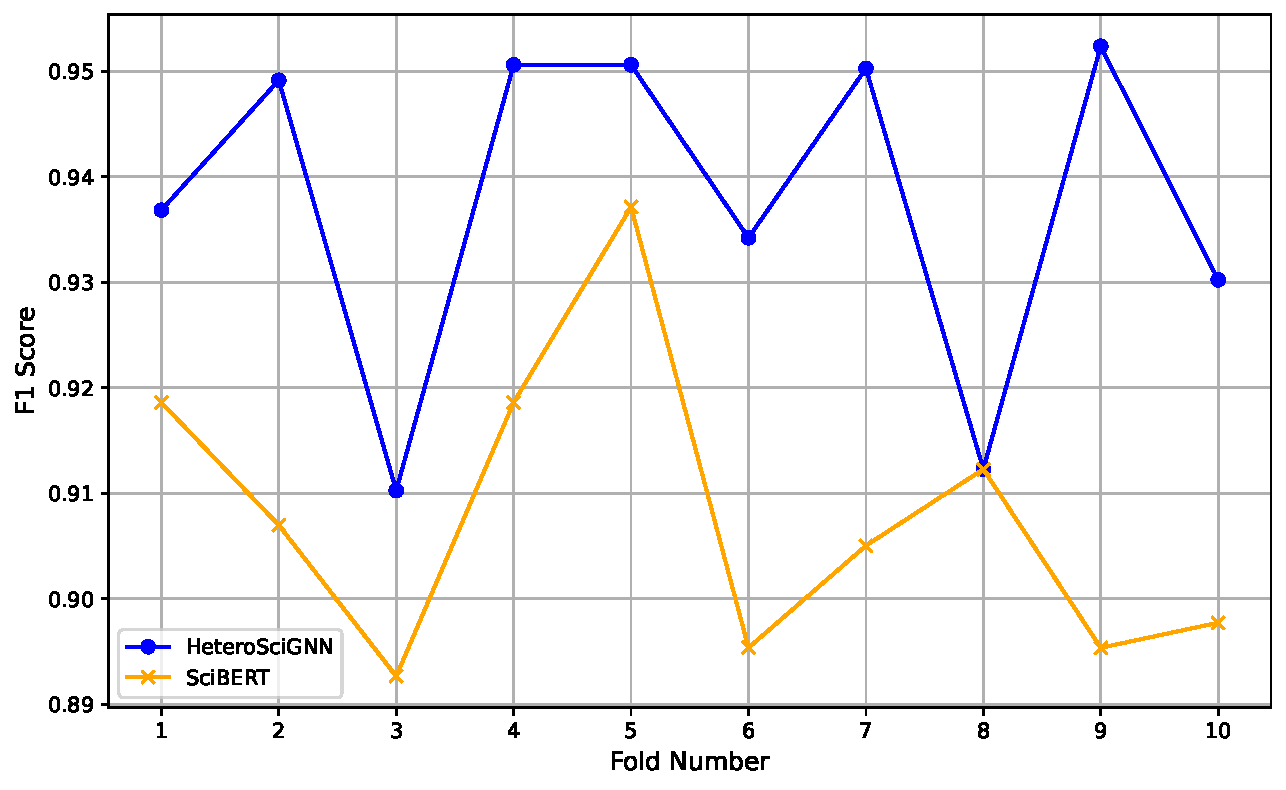
\includegraphics[width=\linewidth]{Figures/Comparison_F1_Scores_2_models.pdf}
   \caption{
    Comparison of F1-scores between the DruGNNosis-MoA and our fine-tuned SciBERT models.
   Each point on the lines corresponds to the F1-score obtained for that particular fold of the cross-validation.
   DruGNNosis-MoA model outperformed our fine-tuned SciBERT on a fold-by-fold basis.}
\label{fig:fscore1}
\end{figure}



\newpage
%-------------------
\section{Supplementary Tables}
\label{sec11}
%-------------------

%-------------------
%{Supplementary Table S1}
%-------------------
\subsection{Supplementary Table S1} 
Table S1 can be accessed through: 
\url{https://github.com/Anonymousv123/DruGNNosis-MoA/tree/main/Supplementary}
%\url{https://github.com/bartala/PalliativEtiological/tree/main/Supplementary}.
Tab 1 contains drug mechanism annotations.
Tab 2 contains example drug mechanism.


%-------------------
%{Supplementary Table S2}
%-------------------
\subsection{Supplementary Table S2}

\begin{table}[h!]
\centering
\begin{threeparttable}
\caption*{Table S2: Training configurations of baseline GNNs.}
\label{tbl:cv_scores}
\begin{tabular}{@{\extracolsep\fill} p{0.07\textwidth} p{0.4\textwidth} @{\extracolsep\fill}}
\toprule
Model & Configuration \\
\midrule
SAGEConv & 
    Two SageConv layers, ReLU activation, and an Adam optimizer (learning rate \(5 \times 10^{-4}\)) with gradient clipping at 0.5, and 100 epochs, using EigenVector-based node features.
\\
GATConv+ Fine-tuned SciBERT &  
    Two GATConv layers with multi-head attention followed by ReLU activation. 
    An Adam optimizer with a learning rate of \(5 \times 10^{-4}\) and gradient clipping at 0.5.
    The model was trained over 100 epochs, using fine-tuned SciBERT embeddings as node features.
\\
GATConv & 
    Two GATConv layers with multi-head attention, followed by ReLU activation.
    An Adam optimizer with a learning rate of \(5 \times 10^{-4}\) and gradient clipping at 0.5. The model was trained over 100 epochs using Eigenvector centrality as node features.
\\
GATv2Conv+ Fine-tuned SciBERT &
    Two GATv2Conv layers, utilizing adaptive multi-head attention followed by ReLU activation. 
    An Adam optimizer with a learning rate of \(5 \times 10^{-4}\) and gradient clipping at 0.5.
    The model was trained over 100 epochs, using fine-tuned SciBERT embeddings as node features.
\\
GATv2Conv & 
    Two GATv2Conv layers, utilizing adaptive multi-head attention followed by ReLU activation. 
    An Adam optimizer with a learning rate of \(5 \times 10^{-4}\) and gradient clipping at 0.5. The model was trained over 100 epochs, using Eigenvector centrality as node features.
\\
GraphConv+ Fine-tuned SciBERT & 
    Two GraphConv layers followed by ReLU activation. 
    An Adam optimizer with a learning rate of \(5 \times 10^{-4}\) and gradient clipping at 0.5.
    The model was trained over 100 epochs, using fine-tuned SciBERT embeddings as node features.
\\
GraphConv &  
    Two GraphConv layers to aggregate neighborhood information, followed by ReLU activation. 
    An Adam optimizer with a learning rate of \(5 \times 10^{-4}\) and gradient clipping at 0.5.
    The model was trained over 100 epochs, using Eigenvector centrality as node features.
\\
\bottomrule
\end{tabular}
\begin{tablenotes}
\item Note: Each cross-validation fold used a 90-10 split of the data for training and validation, respectively.
\end{tablenotes}
\end{threeparttable}
\end{table}


%-------------------
%{Supplementary Table S3}
%-------------------
%\subsection{Supplementary File S1}

%A list of publications that support our strategy for classifying drugs as having etiological or palliative mechanisms is provided: 
%\url{https://github.com/Anonymousv123/DruGNNosis-MoA/blob/main/Supplementary/List%20of%20Publications%20Supporting%20Etiological%20vs%20Palliative%20Drug%20Mechanisms_v1_11-24-2024%20(1).pdf}

%\url{https://github.com/Anonymousv123/DruGNNosis-MoA/blob/main/Supplementary/drug_TestSet_predictions_value_genes_associated%20-%20drug_test_predictions_value_genes_associated.csv}




%\end{appendices}

\end{document}
